%This is a very basic  BE PROJECT PRELIMINARY template.

%############################################# 
%#########Author :  PROJECT###########
%#########COMPUTER ENGINEERING############


\documentclass[oneside,a4paper,12pt]{report}
%\usepackage{showframe}
%\hoffset = 8.9436619718309859154929577464789pt
%\voffset = 13.028169014084507042253521126761pt

\fancypagestyle{plain}{%
  \fancyhf{}
  \fancyfoot[CE]{College_Name, Department of Computer Engineering 2015-16}
  \fancyfoot[RE]{\thepage}
}
\pagestyle{fancy}
\fancyhead{}
\renewcommand{\headrulewidth}{0pt}
\footskip = 0.625in
\cfoot{}
\rfoot{}

\usepackage[]{hyperref}
\usepackage{tikz}
\usetikzlibrary{arrows,shapes,snakes,automata,backgrounds,petri}

\usepackage{tabularx}

\usepackage[nottoc,notlot,notlof,numbib]{tocbibind}
\usepackage[titletoc]{appendix}
\usepackage{titletoc}
\renewcommand{\appendixname}{Annexure}
\renewcommand{\bibname}{References}

\setcounter{secnumdepth}{5}

\usepackage{float}
\usepackage{subcaption}
\usepackage{multirow}

\usepackage[ruled,vlined]{algorithm2e}

\begin{document}

\setlength{\parindent}{0mm}
\begin{center}
{\bfseries SAVITRIBAI PHULE PUNE UNIVERSITY \\}
 \vspace*{1\baselineskip}
{\bfseries A  PROJECT REPORT ON \\}
 \vspace*{2\baselineskip}
{\bfseries \fontsize{16}{12} \selectfont  PROJECT TITLE \\ \vspace*{2\baselineskip}}
{\fontsize{12}{12} \selectfont SUBMITTED TOWARDS THE
 \\PARTIAL FULFILLMENT OF THE REQUIREMENTS OF \\

\vspace*{2\baselineskip}}
{\bfseries \fontsize{14}{12} \selectfont BACHELOR OF ENGINEERING (Computer
Engineering) \\
\vspace*{1\baselineskip}} 
{\bfseries \fontsize{14}{12} \selectfont BY \\ 
\vspace*{1\baselineskip}} 
Student Name  \hspace{25 mm} Exam No:  \\
Student Name \hspace{25 mm} Exam No:   \\
Student Name \hspace{25 mm} Exam No:  \\
Student Name \hspace{25 mm} Exam No:\\
\vspace*{2\baselineskip}
{\bfseries \fontsize{14}{12} \selectfont Under The Guidance of \\  
\vspace*{2\baselineskip}} 
Prof. Guide Name\\

\includegraphics[width=100pt]{collegelogo.png} \\
{\bfseries \fontsize{14}{12} \selectfont DEPARTMENT OF COMPUTER ENGINEERING \\
College Name \\
College Address 
}
\end{center}

\newpage



\begin{figure}[ht]
\centering

\includegraphics[width=100pt]{collegelogo.png}
\end{figure}


{\bfseries \fontsize{14}{12} \selectfont \centerline{College Name}
\centerline{DEPARTMENT OF COMPUTER ENGINEERING}
\vspace*{2\baselineskip}} 


{\bfseries \fontsize{16}{12} \selectfont \centerline{CERTIFICATE} 
\vspace*{2\baselineskip}} 

\centerline{This is to certify that the Project Entitled}
\vspace*{.5\baselineskip} 


{\bfseries \fontsize{14}{12} \selectfont \centerline{ PROJECT TITLE}
\vspace*{0.5\baselineskip}}

\centerline{Submitted by}
\vspace*{0.5\baselineskip} 
\centerline{Student Name  \hspace{25 mm} Exam No: } 
\centerline{Student Name \hspace{25 mm} Exam No:  } 
\centerline{Student Name \hspace{25 mm} Exam No: }
\centerline{Student Name \hspace{25 mm} Exam No: }

is a bonafide work carried out by Students under the supervision of Prof. Guide Name and it
is submitted towards the partial fulfillment of the requirement of Bachelor of Engineering (Computer Engineering).\\

\bgroup
\def\arraystretch{0.7}
\begin{tabular}{c c }
Prof. Guide Name &  \hspace{50 mm} Prof. HOD Name \\								
Internal Guide   &  \hspace{50 mm} H.O.D \\
Dept. of Computer Engg.  &	\hspace{50 mm}Dept. of Computer Engg.  \\
\end{tabular}
%}
\begin{center}
%\fontsize{12}{18}\selectfont 
{
Dr. A. V. Deshpande \\
Principal\\
Smt.Kashibai Navale College of Engineering  
}
\end{center}
\\\\
Signature of Internal Examiner \hspace{30 mm} Signature of External Examiner
\newpage
\begin{center}
\textbf{PROJECT APPROVAL SHEET}
\end{center}
\begin{center}
 A Project Title
 \end{center} \\
\begin{center}
(Project Title)
\end{center}\\
\begin{center}
Is successfully completed by 
\end{center}
\centerline{Student Name  \hspace{25 mm} Exam No: } 
\centerline{Student Name \hspace{25 mm} Exam No:  } 
\centerline{Student Name \hspace{25 mm} Exam No: }
\centerline{Student Name \hspace{25 mm} Exam No: }
\begin{center}
 at
 \end{center} 
 \begin{center}
 DEPARTMENT OF COMPUTER ENGINEERING
 \end{center}
 \begin{center}
 (COLLEGE NAME)
 \end{center}
 \begin{center}
 SAVITRIBAI PHULE PUNE UNIVERSITY,PUNE
 \end{center}
 
 \begin{center}
 ACADEMIC YEAR 2015-2016
 \end{center}
 
 \vspace*{1\baselineskip}}
 \begin{tabular}{c c }
Prof. Guide Name &  \hspace{50 mm} Prof. HOD Name \\								
Internal Guide   &  \hspace{50 mm} H.O.D \\
Dept. of Computer Engg.  &	\hspace{50 mm}Dept. of Computer Engg.  \\
\end{tabular}
\newpage

%\pictcertificate{TITLE OF BE PROJECT}{Student Name}{Exam Seat No}{Guide Name}
\setcounter{page}{0}
\frontmatter
\cfoot{College Short Form Name, Department of Computer Engineering 2015-16}
\rfoot{\thepage}
\pagenumbering{Roman}
%\pictack{BE PROJECT TITLE}{Guide Name}

		
{  \newpage {\bfseries \fontsize{14}{12} \selectfont \centerline{Abstract} 
\vspace*{2\baselineskip}} \setlength{\parindent}{11mm} }
{ \setlength{\parindent}{0mm} }
Please Write here One Page Abstract. It should mainly include introduction, motivation,outcome and innovation if any.


{  \newpage {\bfseries \fontsize{14}{12} \selectfont \centerline{Acknowledgments} 
\vspace*{2\baselineskip}} \setlength{\parindent}{11mm} }
{ \setlength{\parindent}{0mm} }
Please Write here Acknowledgment.Example given as\\
\textit{It gives us great pleasure in presenting the preliminary project report 
on {\bfseries \fontsize{12}{12} \selectfont `BE PROJECT TITLE'}.}
\vspace*{1.5\baselineskip}

 \textit{I would like to take this opportunity to thank my internal guide
 \textbf{Prof. Guide Name} for giving me all the help and guidance I needed. I am
 really grateful to them for their kind support. Their valuable suggestions were very helpful.} \vspace*{1.5\baselineskip}

 \textit{I am also grateful to \textbf{Prof. HOD Name}, Head of Computer
 Engineering Department, CollegeName for his indispensable
 support, suggestions.}
\vspace*{1.5\baselineskip}

\textit{In the end our special thanks to \textbf{Other Person Name} for
providing various resources such as  laboratory with all needed software platforms,
continuous Internet connection, for Our Project.}
\vspace*{3\baselineskip} \\
\begin{tabular}{p{8.2cm}c}
&Student Name1\\
&Student Name2\\
&Student Name3\\
&Student Name4\\
&(B.E. Computer Engg.)
%}
\end{tabular}


% \maketitle
\tableofcontents
\listoffigures 
\listoftables



\mainmatter



  \titleformat{\chapter}[display]
{\fontsize{16}{15}\filcenter}
{\vspace*{\fill}
 \bfseries\LARGE\MakeUppercase{\chaptertitlename}~\thechapter}
{1pc}
{\bfseries\LARGE\MakeUppercase}
[\thispagestyle{empty}\vspace*{\fill}\newpage]







\setlength{\parindent}{11mm}
\chapter{Synopsis}

\section{Project Title}
 Project Title

\section{ Project Option }
Please mention type either industry sponsored, entrepreneur or internal project

\section{Internal Guide}
Prof. Internal Guide Name

\section{ Sponsorship and External Guide} 
Please write if any sponsorship


\section{Technical Keywords (As per ACM Keywords)}
% {\bfseries Technical Key Words:}      
% \begin{itemize}
%   \item 	Cloud Computing
% \item	Service Composition
% \item	Online Web services
% \end{itemize}
Please note ACM Keywords can be found : http://www.acm.org/about/class/ccs98-html \\
Example is given as
\begin{enumerate}
	\item C. Computer Systems Organization 
	\begin{enumerate}
		\item C.2 COMPUTER-COMMUNICATION NETWORKS 
		\begin{enumerate}
			\item C.2.4 Distributed Systems 
			\begin{enumerate}
				\item  Client/server 
\item Distributed applications
\item Distributed databases
\item Network operating systems 
\item Distributed file systems
\item Security and reliability issues in distributed applications
	 		\end{enumerate} 
		\end{enumerate} 
	  

	
	\end{enumerate}
\end{enumerate}



\section{Problem Statement}
\label{sec:problem}
        Define Problem Statement
\section{Abstract}
\begin{itemize}
	\item Abstract (10 to 15 lines)
\end{itemize}

\section{Goals and Objectives}
\begin{itemize}
	\item Objectives
\end{itemize}

	
\section{Relevant mathematics associated with the Project}
\label{sec:math}
System Description:
\begin{itemize} 
\item Input:	 
\item Output:	 
\item Identify data structures, classes, divide and conquer strategies to exploit distributed/parallel/concurrent processing, constraints. 
\item Functions : Identify Objects, Morphisms, Overloading in functions, Functional relations
\item Mathematical formulation if possible
\item Success Conditions:	 
\item Failure Conditions:		
\end{itemize}


\section{Names of Conferences / Journals where papers can be published}
\begin{itemize}
\item  IEEE/ACM Conference/Journal 1 
\item  Conferences/workshops in IITs
\item  Central Universities or SPPU Conferences 
\item IEEE/ACM Conference/Journal 2 
\end{itemize}


\section{Review of Conference/Journal Papers supporting Project idea}
\label{sec:survey}
   Atleast 10 papers + White papers or web references\\
   Brief literature survey [ Description containing important description of at least 10 papers

\section{Plan of Project Execution}
  Using planner or alike project management tool.



\chapter{Technical Keywords}
\section{Area of Project}
Project Area

\section{Technical Keywords}
% {\bfseries Technical Key Words:}      
% \begin{itemize}
%   \item 	Cloud Computing
% \item	Service Composition
% \item	Online Web services
% \end{itemize}
Please note ACM Keywords can be found : http://www.acm.org/about/class/ccs98-html \\
Example is given as

\begin{enumerate}
	\item C. Computer Systems Organization 
	\begin{enumerate}
		\item C.2 COMPUTER-COMMUNICATION NETWORKS 
		\begin{enumerate}
			\item C.2.4 Distributed Systems 
			\begin{enumerate}
				\item  Client/server 
\item Distributed applications
\item Distributed databases
\item Network operating systems 
\item Distributed file systems
\item Security and reliability issues in distributed applications
	 		\end{enumerate} 
		\end{enumerate} 
	  

	
	\end{enumerate}
\end{enumerate}

			
\chapter{Introduction}
\section{Project Idea}
\begin{itemize}
\item Project Idea
\end{itemize}


\section{Motivation of the Project}  
\begin{itemize}
\item Motivation of the Project
\end{itemize}

\section{Literature Survey}
\begin{itemize}
\item Review of the papers, Description , Mathematical Terms 
\end{itemize}


\chapter{Problem Definition and scope}
\section{Problem Statement}
Description of Problem


\subsection{Goals and objectives}  
Goal and Objectives: 
\begin{itemize}
  	\item Overall goals and objectives of software, input and output description with necessary syntax, format etc are described
\end{itemize}

 \subsection{Statement of scope} 
	\begin{itemize}  
	\item	A description of the software with Size of input, bounds on input, input validation, input dependency, i/o state diagram, Major inputs, and outputs are described without regard to implementation detail.
	\item The scope identifies what the product is and is not, what it will and won’t do, what it will and wont contain.
	\end{itemize}


\section{Major Constraints}
\begin{itemize}
\item Any constraints that will impact the manner in which the software is to be specified, designed, implemented or tested are noted here.
\end{itemize}

\section{Methodologies of Problem solving and efficiency issues}
\begin{itemize}
	\item The single problem can be solved by different solutions.  This considers the performance parameters for each approach. Thus considers the efficiency issues.
\end{itemize}



\section{Outcome}
\begin{itemize}
\item Outcome of the project
\end{itemize}

\section{Applications}
\begin{itemize}
\item Applications of Project
\end{itemize}

\section{Hardware Resources Required}
\begin{table}[!htbp]
\begin{center}
\def\arraystretch{1.5}
  \begin{tabular}{| c | c | c | c |}
\hline
Sr. No. &	Parameter &	Minimum Requirement & Justification \\
\hline
1 &	CPU Speed &	 2 GHz  & Remark Required\\
\hline
2 &	RAM  &	3 GB &  Remark Required\\
 \hline
\end{tabular}
 \caption { Hardware Requirements }
 \label{tab:hreq}
\end{center}

\end{table}


\section{Software Resources Required}
Platform : 
\begin{enumerate}
\item Operating System: 
\item IDE: 
\item Programming Language
\end{enumerate}




\chapter{Project Plan}

\section{Project Estimates}
                 Use Waterfall model and associated streams derived from assignments 1,2, 3, 4 and 5( Annex A and B) for estimation. 
\subsection{Reconciled Estimates}
\subsubsection{Cost Estimate}

\subsubsection{Time Estimates}


\subsection{Project Resources}
          Project resources  [People, Hardware, Software, Tools and other resources] based on Memory Sharing, IPC, and Concurrency derived using appendices to be referred. 

\section{Risk Management w.r.t. NP Hard analysis}
This section discusses Project risks and the approach to managing them.
\subsection{Risk Identification}
For risks identification, review of scope document, requirements specifications and schedule is done. Answers to questionnaire revealed some risks. Each risk is categorized as per the categories mentioned in \cite{bookPressman}. Please refer table \ref{tab:risk} for all the risks. You can refereed following risk identification questionnaire.

\begin{enumerate}
\item Have top software and customer managers formally committed to support the project?
\item Are end-users enthusiastically committed to the project and the system/product to be built?
\item Are requirements fully understood by the software engineering team and its customers?
\item Have customers been involved fully in the definition of requirements?
\item Do end-users have realistic expectations?
\item Does the software engineering team have the right mix of skills?
\item Are project requirements stable?
\item Is the number of people on the project team adequate to do the job?
\item Do all customer/user constituencies agree on the importance of the project and on the requirements for the system/product to be built?
\end{enumerate}

\subsection{Risk Analysis}
The risks for the Project can be analyzed within the constraints of time and quality

\begin{table}[!htbp]
\begin{center}
%\def\arraystretch{1.5}
\def\arraystretch{1.5}
\begin{tabularx}{\textwidth}{| c | X | c | c | c | c |}
\hline
\multirow{2}{*}{ID} & \multirow{2}{*}{Risk Description}	& \multirow{2}{*}{Probability} & \multicolumn{3}{|c|}{Impact} \\ \cline{4-6}
	& & &	Schedule	& Quality	& Overall \\ \hline
1	& Description 1	& Low	& Low	& High	& High \\ \hline
2	& Description 2	& Low	& Low	& High	& High \\ \hline
\end{tabularx}
\end{center}
\caption{Risk Table}
\label{tab:risk}
\end{table}


\begin{table}[!htbp]
\begin{center}
%\def\arraystretch{1.5}
\def\arraystretch{1.5}
\begin{tabular}{| c | c | c |}
\hline
Probability & Value &	Description \\ \hline
High &	Probability of occurrence is &  $ > 75 \% $ \\ \hline
Medium &	Probability of occurrence is  & $26-75 \% $ \\ \hline
Low	& Probability of occurrence is & $ < 25 \% $ \\ \hline
\end{tabular}
\end{center}
\caption{Risk Probability definitions \cite{bookPressman}}
\label{tab:riskdef}
\end{table}

\begin{table}[!htbp]
\begin{center}
%\def\arraystretch{1.5}
\def\arraystretch{1.5}
\begin{tabularx}{\textwidth}{| c | c | X |}
\hline
Impact & Value	& Description \\ \hline
Very high &	$> 10 \%$ & Schedule impact or Unacceptable quality \\ \hline
High &	$5-10 \%$ & Schedule impact or Some parts of the project have low quality \\ \hline
Medium	& $ < 5 \% $ & Schedule impact or Barely noticeable degradation in quality Low	Impact on schedule or Quality can be incorporated \\ \hline
\end{tabularx}
\end{center}
\caption{Risk Impact definitions \cite{bookPressman}}
\label{tab:riskImpactDef}
\end{table}

\subsection{Overview of Risk Mitigation, Monitoring, Management}


Following are the details for each risk.
\begin{table}[!htbp]
\begin{center}
%\def\arraystretch{1.5}
\def\arraystretch{1.5}
\begin{tabularx}{\textwidth}{| l | X |}
\hline 
Risk ID	& 1 \\ \hline
Risk Description	& Description 1 \\ \hline
Category	& Development Environment. \\ \hline
Source	& Software requirement Specification document. \\ \hline
Probability	& Low \\ \hline
Impact	& High \\ \hline
Response	& Mitigate \\ \hline
Strategy	& Strategy \\ \hline
Risk Status	& Occurred \\ \hline
\end{tabularx}
\end{center}
%\caption{Risk Impact definitions \cite{bookPressman}}
\label{tab:risk1}
\end{table}

\begin{table}[!htbp]
\begin{center}
%\def\arraystretch{1.5}
\def\arraystretch{1.5}
\begin{tabularx}{\textwidth}{| l | X |}
\hline 
Risk ID	& 2 \\ \hline
Risk Description	& Description 2 \\ \hline
Category	& Requirements \\ \hline
Source	& Software Design Specification documentation review. \\ \hline
Probability	& Low \\ \hline
Impact	& High \\ \hline
Response	& Mitigate \\ \hline
Strategy	& Better testing will resolve this issue.  \\ \hline
Risk Status	& Identified \\ \hline
\end{tabularx}
\end{center}
\label{tab:risk2}
\end{table}

\begin{table}[!htbp]
\begin{center}
%\def\arraystretch{1.5}
\def\arraystretch{1.5}
\begin{tabularx}{\textwidth}{| l | X |}
\hline 
Risk ID	& 3 \\ \hline
Risk Description	& Description 3 \\ \hline
Category	& Technology \\ \hline
Source	& This was identified during early development and testing. \\ \hline
Probability	& Low \\ \hline
Impact	& Very High \\ \hline
Response	& Accept \\ \hline
Strategy	& Example Running Service Registry behind proxy balancer  \\ \hline
Risk Status	& Identified \\ \hline
\end{tabularx}
\end{center}
\label{tab:risk3}
\end{table}

\section{Project Schedule}  
\subsection{Project task set}  
Major Tasks in the Project stages are:
\begin{itemize}
  \item Task 1:
  \item Task 2: 
  \item Task 3: 
  \item Task 4: 
  \item Task 5: 
\end{itemize}

\subsection{Task network}  
Project tasks and their dependencies are noted in this diagrammatic form.
\subsection{Timeline Chart}  
A project timeline chart is presented. This may include a time line for the entire project.
Above points should be covered  in Project Planner as Annex C and you can mention here Please refer Annex C for the planner

 
\section{Team Organization}
The manner in which staff is organized and the mechanisms for reporting are noted.  
\subsection{Team structure}
The team structure for the project is identified. Roles are defined.

\subsection{Management reporting and communication}
Mechanisms for progress reporting and inter/intra team communication are identified as per assessment sheet and lab time table. 
 
\chapter{Software requirement specification  }

\section{Introduction}
\subsection{Purpose and Scope of Document}
The purpose of SRS and what it covers is to be stated 

\subsection{Overview of responsibilities of Developer}
What all activities carried out by developer?
  
\section{Usage Scenario}
This section provides various usage scenarios for the system to be developed.  
 \subsection{User profiles}  
The profiles of all user categories are described here.(Actors and their Description)

\subsection{Use-cases}
All use-cases for the software are presented. Description of all main Use cases using use case template is to be provided.

\begin{table}[!htbp]
\begin{center}
%\def\arraystretch{1.5}
\def\arraystretch{1.5}
\begin{tabularx}{\textwidth}{| c | c | X | c | X |}
\hline
Sr No.	& Use Case	& Description	& Actors	& Assumptions \\
\hline
1& Use Case 1 & Description & Actors & Assumption \\
\hline
\end{tabularx}
\end{center}
\caption{Use Cases}
\label{tab:usecase}
\end{table}


\subsection{Use Case View}
Use Case Diagram. Example is given below
\begin{center}
	\begin{figure}[!htbp]
		\centering
		\fbox{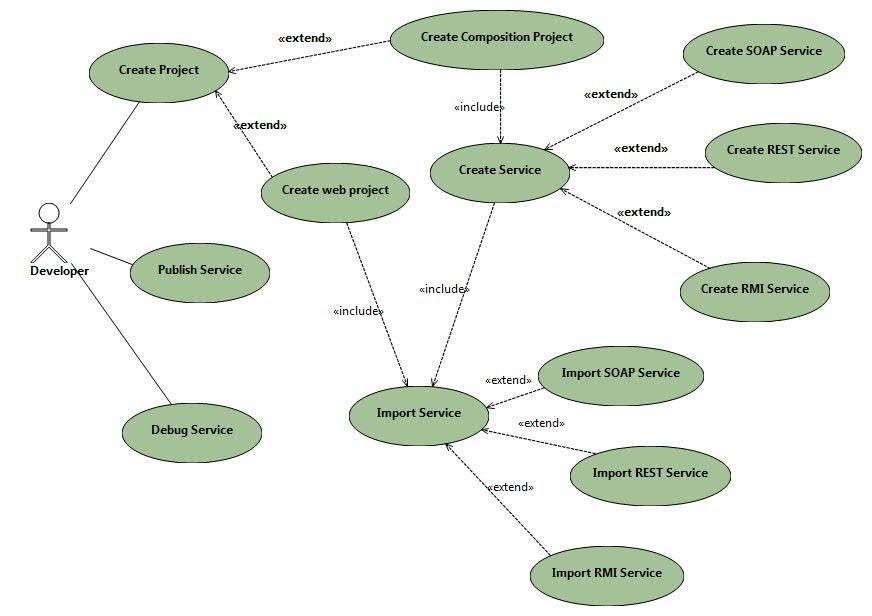
\includegraphics[width=\textwidth]{use-case.jpg}}
	  \caption{Use case diagram}
	  \label{fig:usecase}
	\end{figure}
\end{center}  

\section{Data Model and Description}  
\subsection{Data Description}  
Data objects that will be managed/manipulated by the software are described in this section. The database entities or files or data structures  required to be described. For data objects details can be given as below
\subsection{Data objects and Relationships}
  Data objects and their major attributes and relationships among data objects are described using an ERD- like form.

 
 
\section{Functional Model and Description}  
A description of each major software function, along with data flow (structured analysis) or class hierarchy (Analysis Class diagram with class description for object oriented system) is presented. 
\subsection{Data Flow Diagram}  
\subsubsection{Level 0 Data Flow Diagram}
\subsubsection{Level 1 Data Flow Diagram}
 



 
\subsection{Activity Diagram:}
\begin{itemize}
	\item	The Activity diagram represents the steps taken.
\end{itemize} 

\subsection{Non Functional Requirements:}
\begin{itemize}
	\item	Interface Requirements
	\item	Performance Requirements
    \item	Software quality attributes such as availability [ related to Reliability], modifiability [includes portability, reusability, scalability] ,  		performance, security, testability and usability[includes self 			adaptability and user adaptability] 
\end{itemize} 

\subsection{State Diagram:}	
  State Transition Diagram\\
Fig.\ref{fig:state-dig} example shows the state transition diagram of Cloud SDK. The states are
represented in ovals and state of system gets changed when certain events occur. The transitions from one state to the other are represented by arrows. The Figure    shows important states and events that occur while creating new project.

\begin{center}
	\begin{figure}[!htbp]
		\centering
		\fbox{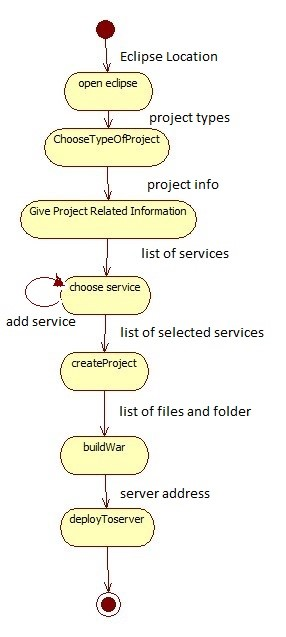
\includegraphics[width=230pt]{state-dig.jpg}}
	  \caption{State transition diagram}
	  \label{fig:state-dig}
	\end{figure}
\end{center} 
 
 \subsection{Design Constraints}	
Any design constraints that will impact the subsystem are noted.
 \subsection{Software Interface Description}	 
The software interface(s)to the outside world is(are) described.
The requirements for interfaces to other devices/systems/networks/human are stated.



\chapter{Detailed Design Document using Appendix A and B}
 \section{Introduction}  
This document specifies the design that is used to solve the problem of Product.  
\section{Architectural Design}  
	A description of the program architecture is presented. Subsystem design or Block diagram,Package Diagram,Deployment diagram with description is to be presented.

 
  \begin{center}
	\begin{figure}[!htbp]
		\centering
		\fbox{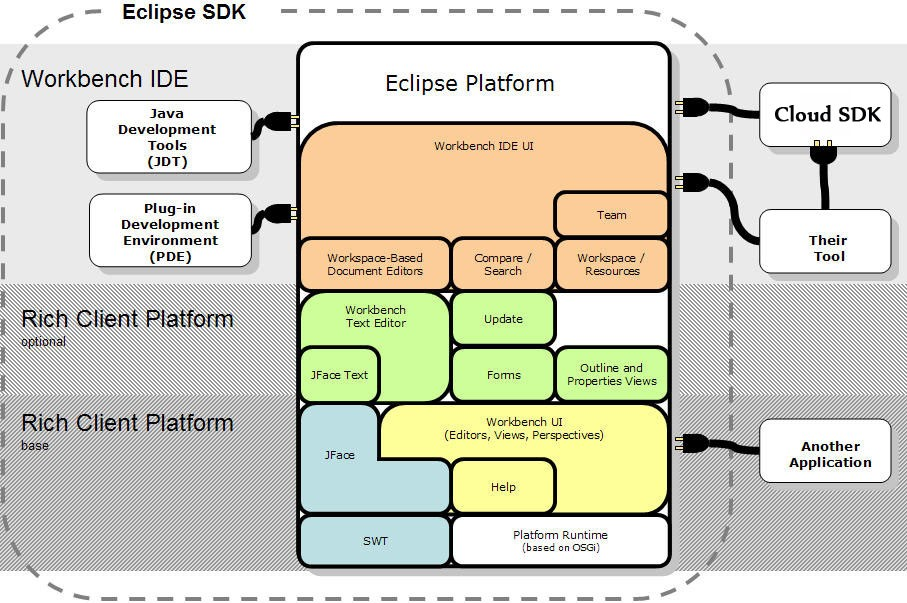
\includegraphics[width=\textwidth]{arch2.jpg}}
	  \caption{Architecture diagram}
	  \label{fig:arch-dig}
	\end{figure}
\end{center} 


\section{Data design (using Appendices A and B)}   
A description of all data structures including internal, global, and temporary data structures, database design (tables), file formats.
\subsection{Internal software data structure}
Data structures that are passed among components the software are described.
\subsection{Global data structure}
Data structured that are available to major portions of the architecture are described.
\subsection{Temporary data structure}
Files created for interim use are described.
\subsection{Database description}
Database(s) / Files created/used  as part of the application is(are) described.


\section{Compoent Design} 
Class diagrams, Interaction Diagrams, Algorithms. Description of each component description required.
\subsection{Class Diagram}
 \begin{center}
	\begin{figure}[!htbp]
		\centering
		\fbox{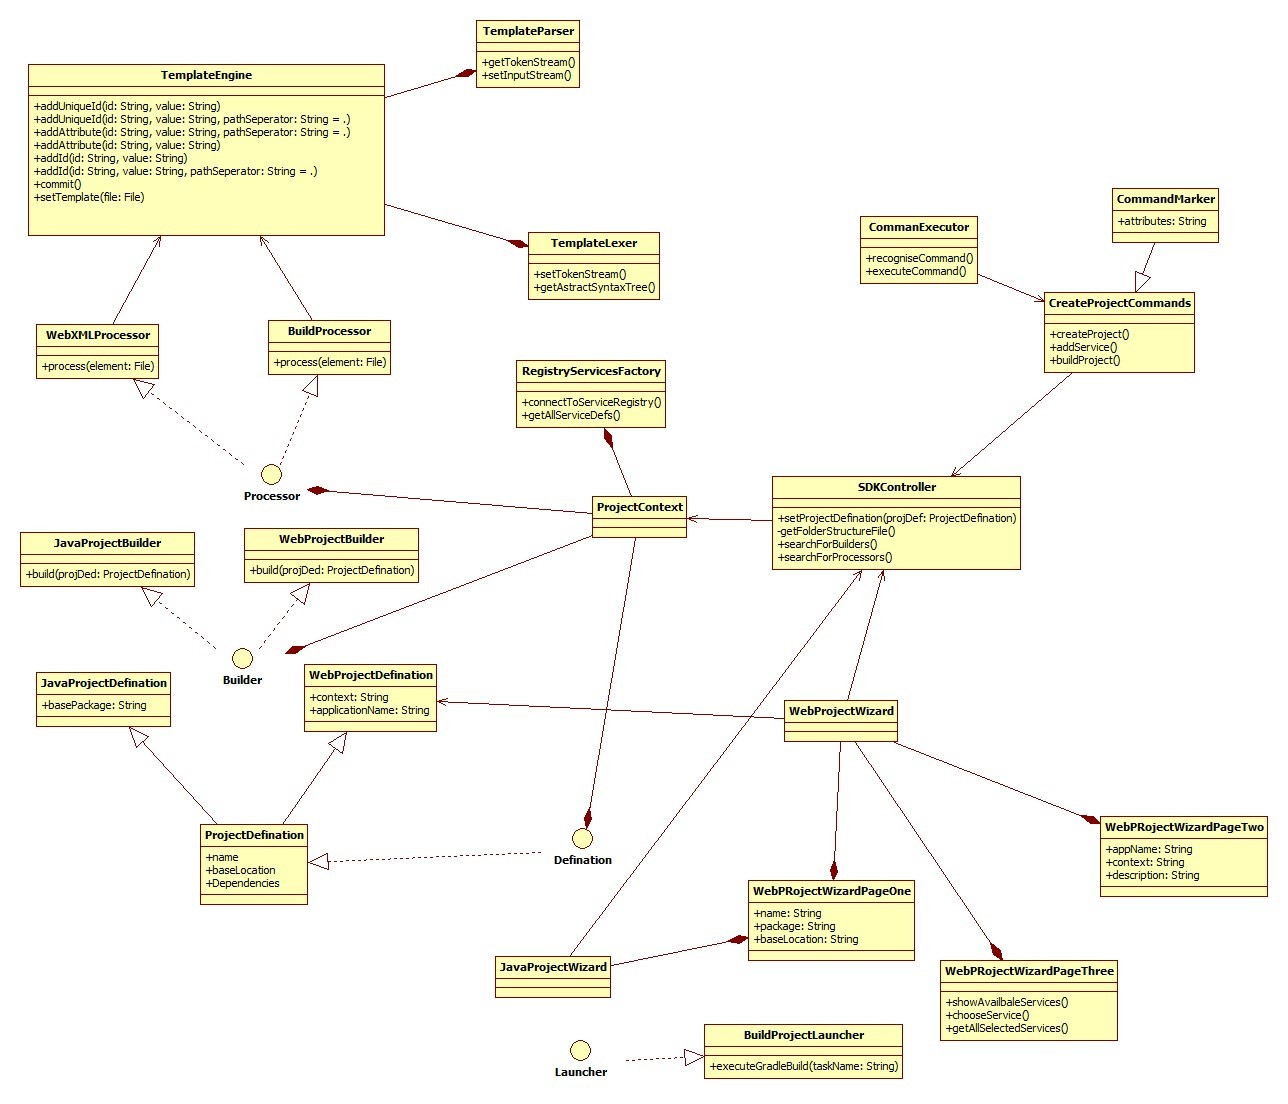
\includegraphics[width=450pt]{class-dig.jpg}}
	  \caption{Class Diagram}
	  \label{fig:class-dig}
	\end{figure}
\end{center} 
 
\chapter{Project Implementation}
  \section{Introduction}
  \section{Tools and Technologies Used}
  \section{Methodologies/Algorithm Details}
  \subsection{Algorithm 1/Pseudo Code}
  \subsection{Algorithm 2/Pseudo Code}
  \section{Verification and Validation for Acceptance}
  
  
\chapter{Software Testing}
 \section{Type of Testing Used}
   Unit,Integration,system etc.
   \section{Test Cases and Test Results}
   for each type of testing done.    
   
\chapter{Results}
\section{Screen shots}
Outputs / Snap shots of the results
\section{Outputs}

    Outputs / Snap shots of the results
\chapter{Deployment and Maintenance}
     \section{Installation and un-installation}
     \section{User help}
     
 \chapter{Conclusion and future scope}
Write  summary , conclusion and future scope
 }
% \bibliographystyle{plain}

\bibliographystyle{ieeetr}
\bibliography{biblo}

\begin{appendices}

\chapter{References}
(Strictly in ACM Format)

% \chapter{ALGORITHMIC DESIGN}
\chapter{Laboratory assignments on Project Analysis of Algorithmic Design}
\begin{itemize}
\item To develop the problem under consideration and justify feasibilty using
concepts of knowledge canvas and IDEA Matrix.\\
Refer \cite{innovationbook} for IDEA Matrix and Knowledge canvas model. Case studies are given in this book. IDEA Matrix is represented in the following form. Knowledge canvas represents about identification  of opportunity for product. Feasibility is represented w.r.t. business perspective.\\ 

\begin{table}[!htbp]
\begin{center}
  \begin{tabular}{| c | c | c | c |}
\hline
 I & D & E & A \\ 
\hline
Increase & Drive & Educate & Accelerate \\
\hline
Improve & Deliver & Evaluate & Associate  \\
 \hline
Ignore & Decrease & Eliminate & Avoid \\
\hline
\end{tabular}
 \caption { IDEA Matrix }
 \label{tab:imatrix}
\end{center}
\end{table}

\item Project problem statement feasibility assessment using NP-Hard, NP-Complete or satisfy ability issues using modern algebra and/or relevant mathematical models.
\item input x,output y, y=f(x)
\end{itemize}

\chapter{Laboratory assignments on Project Quality and Reliability Testing of Project Design}

It should include assignments such as
\begin{itemize}
\item Use of divide and conquer strategies to exploit distributed/parallel/concurrent processing of the above to identify object, morphisms, overloading in functions (if any), and functional relations and any other dependencies (as per requirements).
             It can include Venn diagram, state diagram, function relations, i/o relations; use this to derive objects, morphism, overloading

\item Use of above to draw functional dependency graphs and relevant Software modeling methods, techniques
including UML diagrams or other necessities using appropriate tools.
\item Testing of project problem statement using generated test data (using mathematical models, GUI, Function testing principles, if any) selection and appropriate use of testing tools, testing of UML diagram's reliability. Write also test cases [Black box testing] for each identified functions. 
You can use Mathematica or equivalent open source tool for generating test data. 
\item Additional assignments by the guide. If project type as Entreprenaur, Refer \cite{ehr},\cite{mckinsey},\cite{mckinseyweb}, \cite{govwebsite}
\end{itemize}


\chapter{Project Planner}
\label{app:plan}
Using planner or alike project management tool.




\chapter{Reviewers Comments of Paper Submitted}
(At-least one technical paper must be submitted in Term-I on the project design in the
conferences/workshops in IITs, Central Universities or UoP Conferences or equivalent International Conferences Sponsored by IEEE/ACM)
\begin{enumerate}
\item Paper Title:
\item Name of the Conference/Journal where paper submitted :
\item Paper accepted/rejected : 
\item Review comments by reviewer :
\item Corrective actions if any :  

\end{enumerate}

\chapter{Plagiarism Report}
Plagiarism report
\chapter{ Term-II Project Laboratory Assignments}
\begin{enumerate}
\item Review of design and necessary corrective actions taking into consideration the feedback report of Term I assessment, and other competitions/conferences participated like IIT, Central Universities, University Conferences or equivalent centers of excellence etc.
\item Project workstation selection, installations along with setup and installation report preparations.
\item Programming of the project functions, interfaces and GUI (if any) as per 1 st Term term-work submission using corrective actions recommended in Term-I assessment of Term-work.
\item Test tool selection and testing of various test cases for the project performed and generate various testing result charts, graphs etc. including reliability testing.\\
\textbf{Additional assignments for the Entrepreneurship Project:}
\item Installations and Reliability Testing Reports at the client end.

\end{enumerate}
\chapter{Information of Project Group Members}
one page for each student .
\newpage
\begin{enumerate}
\item Name :  \hspace{90 mm}\includegraphics[width=60pt]{photo.jpg}
\item Date of Birth :
\item Gender : 
\item Permanent Address :
\item E-Mail : 
\item Mobile/Contact No. :
\item Placement Details :
\item Paper Published : 

\end{enumerate}
\end{appendices}


\end{document}
